\subsubsection{Hardware}
\begin{frame}{Hardware optimisation}
Molecular dynamics scales incredibly well with increasing computational power. 
	\begin{tikzpicture}
	\begin{axis}[
	title={Hardware scaling of MD simulations},
	xlabel={Hardware},
	ylabel={Speed (ns day\textsuperscript{-1})},
	width=\textwidth,
	height=0.6\textheight,
	legend pos=south west,
	align=center,
%	x dir=reverse,
	xmin=1-thread, xmax=20-threads,
%	ymin=0, ymax=300,
%	ytick ={0,100,200,300},
	y tick label style={rotate=45,anchor=east,
	/pgf/number format/.cd,%
 	          scaled y ticks = true,
          set thousands separator={},
          fixed,},
    symbolic x coords={1-thread, 4-threads, 8-threads, 10-threads, 16-threads, 20-threads, 1-gpu},
    xtick = {1-thread,4-threads,8-threads,10-threads,16-threads,20-threads,1-gpu},
    x tick label style={rotate=45,anchor=east,
	/pgf/number format/.cd,%
          scaled x ticks = false,
          set thousands separator={},
          fixed,},
	]
	\addplot [mark=x,  ] table [x=x, y=y,] {data/scaling.dat};
	
	\end{axis}
	\end{tikzpicture}

\end{frame}
\begin{frame}{Hardware optimisation}
Molecular dynamics scales incredibly well with increasing computational power. 
	\begin{tikzpicture}
	\begin{axis}[
	title={Hardware scaling of MD simulations},
	xlabel={Hardware},
	ylabel={Speed (ns day\textsuperscript{-1})},
	width=\textwidth,
	height=0.6\textheight,
	legend pos=south west,
	align=center,
%	x dir=reverse,
%	xmin=1-thread, xmax=20-threads,
	ymin=0, ymax=300,
%	ytick ={0,100,200,300},
	y tick label style={rotate=45,anchor=east,
	/pgf/number format/.cd,%
 	          scaled y ticks = true,
          set thousands separator={},
          fixed,},
    symbolic x coords={1-thread, 4-threads, 8-threads, 10-threads, 16-threads, 20-threads, gpu},
    xtick = {1-thread,4-threads,8-threads,10-threads,16-threads,20-threads,gpu},
    x tick label style={rotate=45,anchor=east,
	/pgf/number format/.cd,%
          scaled x ticks = false,
          set thousands separator={},
          fixed,},
	]
	\addplot [mark=x] table [x=x, y=y,] {data/scaling.dat};
	
	\end{axis}
	\end{tikzpicture}

\end{frame}

\begin{frame}{GPU Benchmark}
\begin{columns}
\column{0.5\textwidth}
\begin{figure}
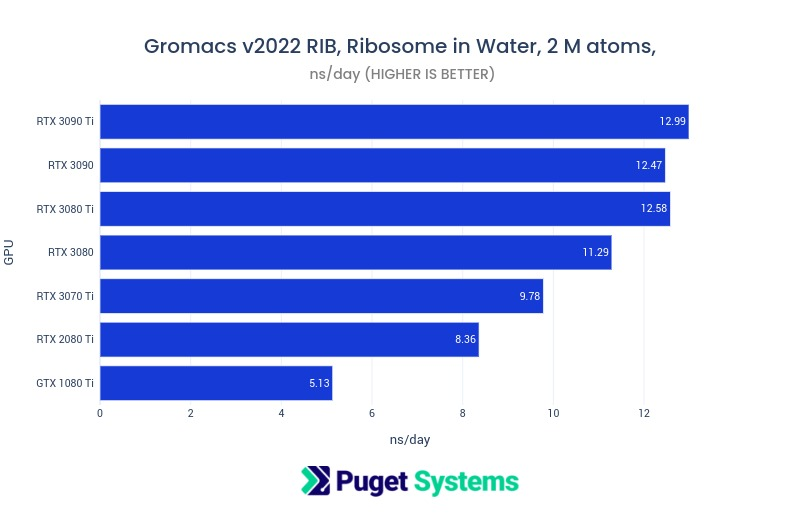
\includegraphics[width=0.95\textwidth]{figures/System/pugetbench.jpeg}
\end{figure}
\column{0.5\textwidth}
\begin{figure}
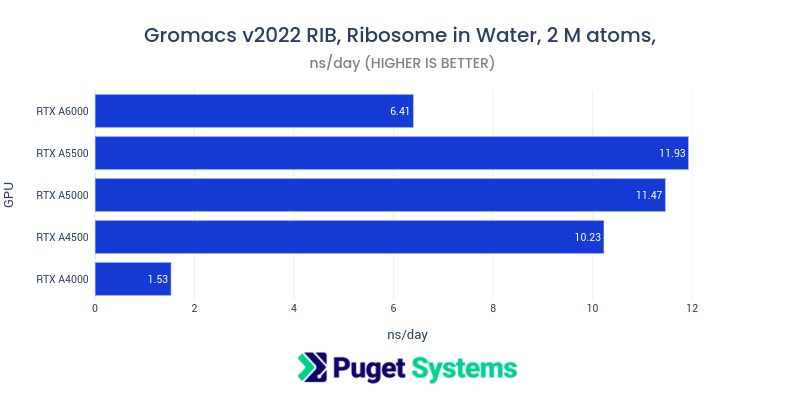
\includegraphics[width=0.95\textwidth]{figures/System/pugetbench_pro.jpeg}
\end{figure}
\end{columns}
Benchmark data: \href{https://www.pugetsystems.com/labs/hpc/molecular-dynamics-benchmarks-gpu-roundup-gromacs-namd2-namd-3alpha-on-12-gpus-2330/}{Puget Systems}
\end{frame}

\subsubsection{Software}
\begin{frame}{Software}
    \begin{table}[H]
    \centering
    \begin{tabular}{@{}cll@{}}
    \toprule
    \multicolumn{1}{l}{\textbf{Section}} & \textbf{Software}  & \textbf{Availability}   \\ \midrule
    Docking         & gnina            		& Open Source	        \\
    Preparation		& acPype				& Free					\\
    Dynamics        & Amber (AmberTools)    & Free*                 \\
    Analysis		& AmberTools			& Free					\\
    Visualisation   & VMD     				& Free for academic use \\
    \bottomrule
    \end{tabular}
    \label{Tab:software}
    \caption{Software}
    \end{table}
* AmberTools is free to use, but full Amber requires a licence. This is only used for GPU acceleration.
\end{frame}